\documentclass[9pt,t]{beamer}
% note that full page width is 12.8 cm and height is 9.6 cm

\mode<presentation>
{
  \usepackage[headline,footline]{beamerthemelectures}

}

% load packages
\usepackage[english]{babel}
\usepackage{graphicx}
\usepackage{multimedia}
%\usepackage[T1]{fontenc}
\usepackage{lmodern}
\usepackage{amsmath,amssymb}
\usepackage{pgf,booktabs,verbatim}
\usepackage{pgfarrows,pgfnodes}
\usepackage[absolute,overlay]{textpos}
\setlength{\TPHorizModule}{\paperwidth}
\setlength{\TPVertModule}{\paperheight}
\usepackage{tikz}

\setbeamertemplate{frametitle}{
\begin{centering}
\insertframetitle
\par
\end{centering}
} 

% create command to add nice looking citation
\newcommand{\reference}[1]{\flushright \vspace{-0.3cm} {\tiny #1}} 


\title{Solutions to Modeling Exercise \#1\\ Introduction to Systems Modeling}

\begin{document}

\section{}

%%%
\frame{
    \frametitle{\vspace{1cm}\huge Introduction to Systems Modeling}   
}

\frame{
\frametitle{1. Set-up model and run to steady-state}
\begin{figure}
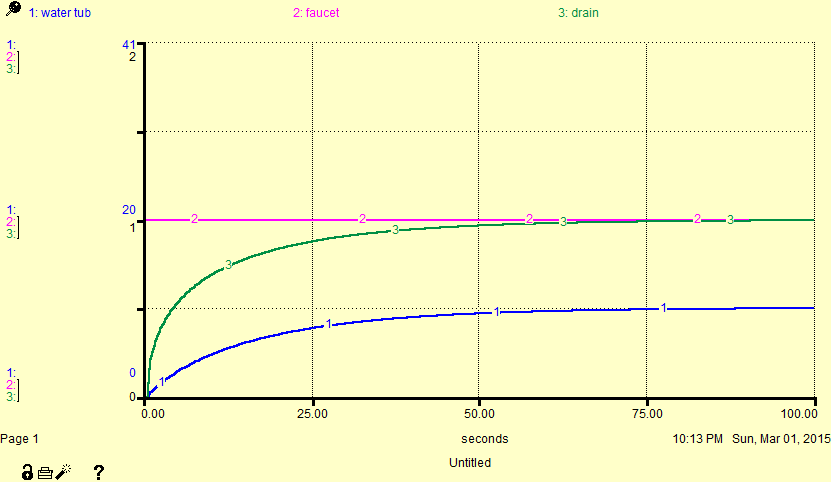
\includegraphics[width=0.9\textwidth]{./p1.jpg}
\end{figure}
}

\frame{
\frametitle{2. Residence times}
\begin{figure}
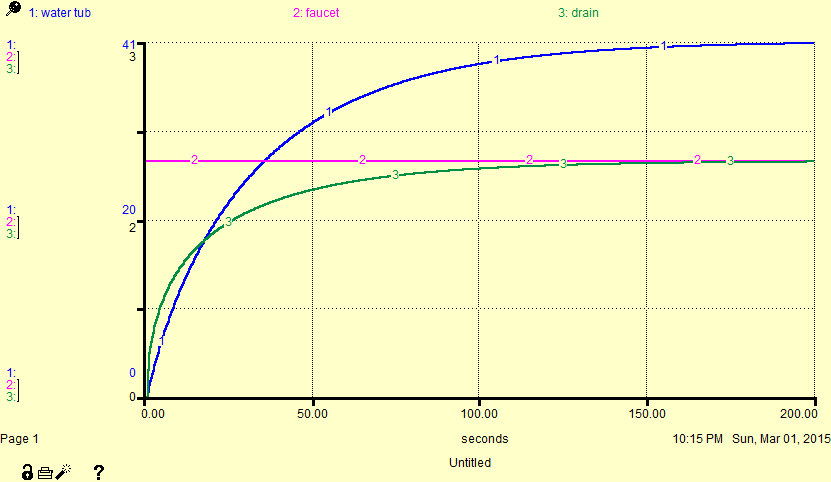
\includegraphics[width=0.9\textwidth]{./p2.jpg}
\end{figure}
\begin{itemize}
\item Residence time = Reservoir volume / inflow
\item Doubling the inflow increase the reservoir by a factor of 4, so the residence time doubled
\end{itemize}
}

\frame{
\frametitle{3. Response times}
\begin{figure}
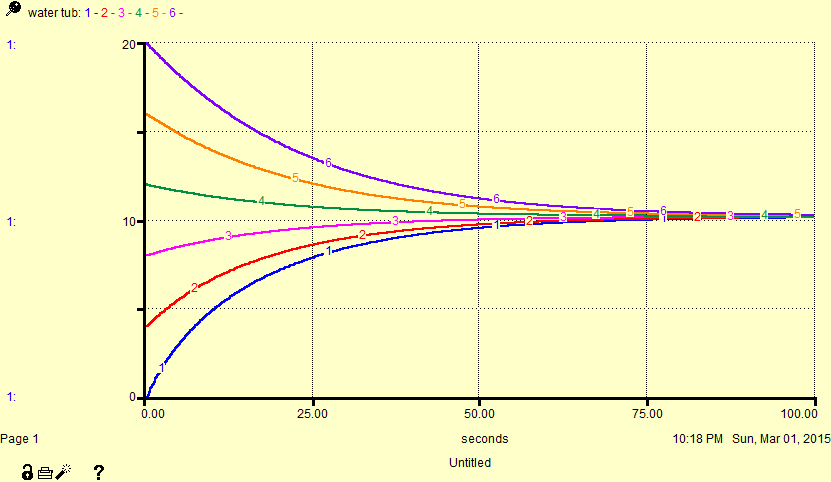
\includegraphics[width=0.9\textwidth]{./p3.jpg}
\end{figure}
\begin{itemize}
\item Longer recovery time for larger perturbation
\item But curvaturve of graphs is similar for all perturbations
\item Note that this model has a strong negative feedback
\end{itemize}
}

\frame{
\frametitle{4. Positive feedback loops}
\begin{figure}
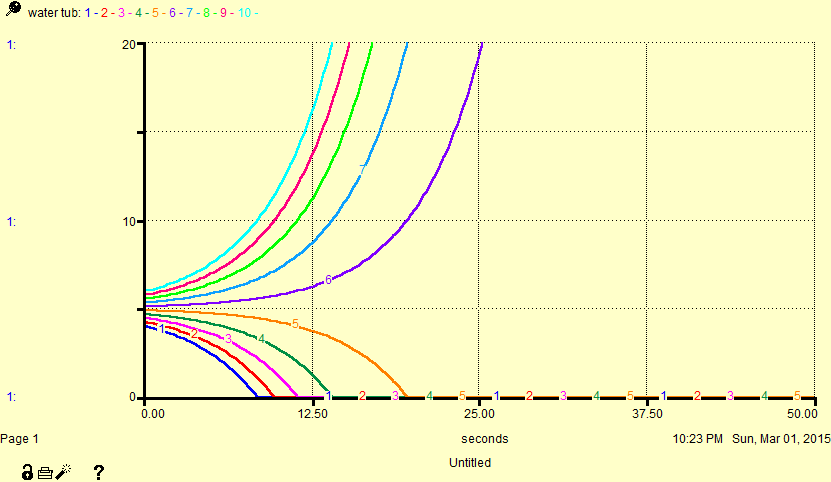
\includegraphics[width=0.9\textwidth]{./p4.jpg}
\end{figure}
\begin{itemize}
\item The model becomes unstable when inflow is proportional to reservoir volume
\end{itemize}
}

\frame{
\frametitle{5. Lag time}
\begin{figure}
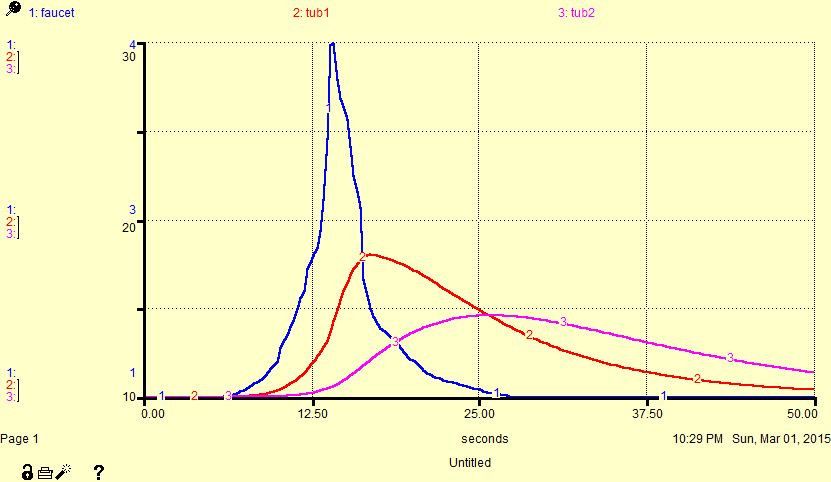
\includegraphics[width=0.9\textwidth]{./p5.jpg}
\end{figure}
\begin{itemize}
\item It takes time for changes to propagate downstream
\item Same total volume of water, but lower peak discharge downstream
\item Commonly observed in many types of systems
\end{itemize}
}


\end{document}